\documentclass[a4paper, 12pt]{article}

%-------------------------%
% PREAMBUŁA --------------%
%-------------------------%
\usepackage[utf8]{inputenc}
\usepackage[OT4]{polski}
\usepackage{caption}
\usepackage{amsmath}
\usepackage{tikz}
\usepackage{subcaption}
\usepackage{tabularx}
%\usepackage{wrapfig}
\usepackage{caption}
\usepackage{array}
\usepackage{hyperref}
\usepackage{graphicx}
%\usepackage{color}
\usepackage{geometry}
%\usepackage{epstopdf}
\usepackage{fancyhdr}
\usepackage{helvet}
\usepackage{graphicx}
\usepackage{color}
%\usepackage{geometry}
\usepackage{physics}
\usepackage{subcaption} 
\usepackage[justification=centering]{caption}
%\usepackage[margin=100pt]{geometry}
\usepackage{bbold}
\usepackage{xparse}

\NewDocumentCommand{\tens}{t_}
 {%
  \IfBooleanTF{#1}
   {\tensop}
   {\otimes}%
 }
\NewDocumentCommand{\tensop}{m}
 {%
  \mathbin{\mathop{\otimes}\displaylimits_{#1}}%
 }
%------- Typy kolumn do ustawiania szerokości ------- %
\newcolumntype{L}[1]{>{\raggedright\let\newline\\\arraybackslash\hspace{0pt}}m{#1}}
\newcolumntype{C}[1]{>{\centering\let\newline\\\arraybackslash\hspace{0pt}}m{#1}}
\newcolumntype{R}[1]{>{\raggedleft\let\newline\\\arraybackslash\hspace{0pt}}m{#1}}

\renewcommand{\arraystretch}{1.3}





 

\geometry{hmargin={2cm, 2cm}, height=10.0in}

\begin{document}

%-------------------------%
%Tabela nagłówkowa -------%
%-------------------------%

\begin{table}[h]
	\centering
	\begin{tabular}{|C{3cm}|L{12cm}|} \hline
		Wydział: \textbf{WFiIS} & Imię i nazwisko: \textbf{Axel Zuziak} \\ \hline
		\textbf{MOFIT 2} & \textbf{Wpływ pola magnetycznego na stany Majorany w nanodrutach półprzewodnikowych.} \\ \hline
	\end{tabular}
\end{table}




\section{Wstęp oraz cel ćwiczenia}

Na cel ćwiczenia składały się dwie symulacje. W pierwszej części przeprowadzono symulację nanodrutu Kitaev'a w celu obserwacji stanów Majorany. Następnie badano obecność stanów Majorany w bardziej skomplikowanym modelu nanodrutu półprzewodnikowego w zależności od zewnętrznego pola magnetycznego. Symulacje zostały zrealizowane w języku Python przy pomocy biblioteki \emph{Kwant}.

\section{Model Kitaev'a}
\subsection{Założenia}

Model nanodrutu Kiteav'a opisany jest Hamiltonianem
\begin{equation}
    H = -\mu \sum_{n=1}^{N} c^{\dag}_n c_n - t\sum_{n=1}^{N} (c^{\dag}_{n+1} c_n + h.c.) + \Delta \sum_{n=1}^{N} (c_n c_{n+1} + h.c.)
    \label{eq:kitaev}
\end{equation}
gdzie $h.c$ oznacza sprzężenie hermitowskie, $\mu$ potencjał chemiczny, $t$ jest energią pomiędzy węzłami, oraz $\Delta$ to superconducting pairing?.

Powyższy Hamiltonian można zapisać w formalizmie Bogoliubov-de Gennes'a
\begin{equation}
    H = \frac{1}{2}C^{\dag} H_{BdG} C
\end{equation}
gdzie $C = (c_1,...,c_n,c^{\dag}_1,...,c^{\dag}_n)^T$.
Macierz $H_{BdG}$ to Hamiltionian Bogoliubov-de Gennes
\begin{equation}
    H_{BdG} = \begin{pmatrix}
        H & \Delta \\
        -\Delta^{*} & -H^{*}
    \end{pmatrix}.
\end{equation}

Aby sformułować Hamiltonian (\ref{eq:kitaev}) w formalizmie Bogoliubov-de Gennes wygodnie jest zapisać macierz $2N \times 2N$ $H_{BdG}$ używając macierzy Pauliego $\tau$ w przestrzeni cząstka-dziura i oznaczając $\ket{n}$ jako wektor $(0,...,1,0,...)^{T}$. Wtedy:
\begin{equation}
    H_{BdG} = -\sum_n \mu \tau_z \ket{n} \bra{n} - \sum_n \left[ (t\tau_z + i\Delta\tau_y) \ket{n} \bra{n+1} + h.c.\right]
\end{equation}

\subsection{Wyniki symulxtacji}
Na wykresie \ref{fig:kitaev_plot}. przedstawiono widmo energii w zależności od potencjału chemicznego. Widmo to pokazuje stany energetyczne odpowiadające danym parametrom. Wyniki te otrzymano tworząc model opisany powyższymi zależnościami o $N = 25$ węzłach, oraz $\Delta = t$.

\begin{figure}[h!]
    \centering
    \fontsize{8}{10}\selectfont % zmniejszam czcionke
    \resizebox{1.0\textwidth}{!}{% GNUPLOT: LaTeX picture with Postscript
\begingroup
  \makeatletter
  \providecommand\color[2][]{%
    \GenericError{(gnuplot) \space\space\space\@spaces}{%
      Package color not loaded in conjunction with
      terminal option `colourtext'%
    }{See the gnuplot documentation for explanation.%
    }{Either use 'blacktext' in gnuplot or load the package
      color.sty in LaTeX.}%
    \renewcommand\color[2][]{}%
  }%
  \providecommand\includegraphics[2][]{%
    \GenericError{(gnuplot) \space\space\space\@spaces}{%
      Package graphicx or graphics not loaded%
    }{See the gnuplot documentation for explanation.%
    }{The gnuplot epslatex terminal needs graphicx.sty or graphics.sty.}%
    \renewcommand\includegraphics[2][]{}%
  }%
  \providecommand\rotatebox[2]{#2}%
  \@ifundefined{ifGPcolor}{%
    \newif\ifGPcolor
    \GPcolortrue
  }{}%
  \@ifundefined{ifGPblacktext}{%
    \newif\ifGPblacktext
    \GPblacktextfalse
  }{}%
  % define a \g@addto@macro without @ in the name:
  \let\gplgaddtomacro\g@addto@macro
  % define empty templates for all commands taking text:
  \gdef\gplbacktext{}%
  \gdef\gplfronttext{}%
  \makeatother
  \ifGPblacktext
    % no textcolor at all
    \def\colorrgb#1{}%
    \def\colorgray#1{}%
  \else
    % gray or color?
    \ifGPcolor
      \def\colorrgb#1{\color[rgb]{#1}}%
      \def\colorgray#1{\color[gray]{#1}}%
      \expandafter\def\csname LTw\endcsname{\color{white}}%
      \expandafter\def\csname LTb\endcsname{\color{black}}%
      \expandafter\def\csname LTa\endcsname{\color{black}}%
      \expandafter\def\csname LT0\endcsname{\color[rgb]{1,0,0}}%
      \expandafter\def\csname LT1\endcsname{\color[rgb]{0,1,0}}%
      \expandafter\def\csname LT2\endcsname{\color[rgb]{0,0,1}}%
      \expandafter\def\csname LT3\endcsname{\color[rgb]{1,0,1}}%
      \expandafter\def\csname LT4\endcsname{\color[rgb]{0,1,1}}%
      \expandafter\def\csname LT5\endcsname{\color[rgb]{1,1,0}}%
      \expandafter\def\csname LT6\endcsname{\color[rgb]{0,0,0}}%
      \expandafter\def\csname LT7\endcsname{\color[rgb]{1,0.3,0}}%
      \expandafter\def\csname LT8\endcsname{\color[rgb]{0.5,0.5,0.5}}%
    \else
      % gray
      \def\colorrgb#1{\color{black}}%
      \def\colorgray#1{\color[gray]{#1}}%
      \expandafter\def\csname LTw\endcsname{\color{white}}%
      \expandafter\def\csname LTb\endcsname{\color{black}}%
      \expandafter\def\csname LTa\endcsname{\color{black}}%
      \expandafter\def\csname LT0\endcsname{\color{black}}%
      \expandafter\def\csname LT1\endcsname{\color{black}}%
      \expandafter\def\csname LT2\endcsname{\color{black}}%
      \expandafter\def\csname LT3\endcsname{\color{black}}%
      \expandafter\def\csname LT4\endcsname{\color{black}}%
      \expandafter\def\csname LT5\endcsname{\color{black}}%
      \expandafter\def\csname LT6\endcsname{\color{black}}%
      \expandafter\def\csname LT7\endcsname{\color{black}}%
      \expandafter\def\csname LT8\endcsname{\color{black}}%
    \fi
  \fi
    \setlength{\unitlength}{0.0500bp}%
    \ifx\gptboxheight\undefined%
      \newlength{\gptboxheight}%
      \newlength{\gptboxwidth}%
      \newsavebox{\gptboxtext}%
    \fi%
    \setlength{\fboxrule}{0.5pt}%
    \setlength{\fboxsep}{1pt}%
\begin{picture}(5102.00,3968.00)%
    \gplgaddtomacro\gplbacktext{%
      \csname LTb\endcsname%
      \put(682,704){\makebox(0,0)[r]{\strut{}$-6$}}%
      \put(682,1204){\makebox(0,0)[r]{\strut{}$-4$}}%
      \put(682,1704){\makebox(0,0)[r]{\strut{}$-2$}}%
      \put(682,2204){\makebox(0,0)[r]{\strut{}$0$}}%
      \put(682,2703){\makebox(0,0)[r]{\strut{}$2$}}%
      \put(682,3203){\makebox(0,0)[r]{\strut{}$4$}}%
      \put(682,3703){\makebox(0,0)[r]{\strut{}$6$}}%
      \put(814,484){\makebox(0,0){\strut{}$0$}}%
      \put(1300,484){\makebox(0,0){\strut{}$0.5$}}%
      \put(1787,484){\makebox(0,0){\strut{}$1$}}%
      \put(2273,484){\makebox(0,0){\strut{}$1.5$}}%
      \put(2760,484){\makebox(0,0){\strut{}$2$}}%
      \put(3246,484){\makebox(0,0){\strut{}$2.5$}}%
      \put(3732,484){\makebox(0,0){\strut{}$3$}}%
      \put(4219,484){\makebox(0,0){\strut{}$3.5$}}%
      \put(4705,484){\makebox(0,0){\strut{}$4$}}%
    }%
    \gplgaddtomacro\gplfronttext{%
      \csname LTb\endcsname%
      \put(176,2203){\rotatebox{-270}{\makebox(0,0){\strut{}$E/t$}}}%
      \put(2759,154){\makebox(0,0){\strut{}$\mu/t$}}%
    }%
    \gplbacktext
    \put(0,0){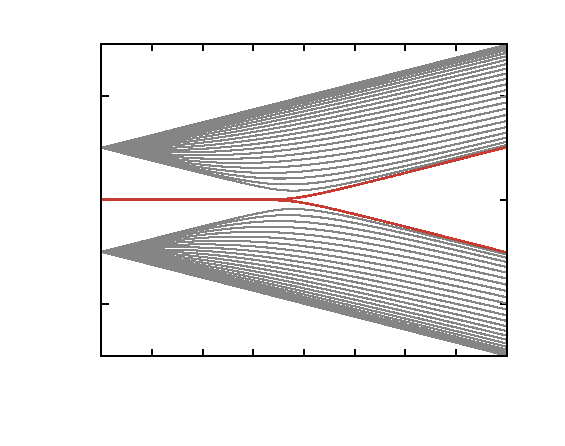
\includegraphics{plots/kitaev}}%
    \gplfronttext
  \end{picture}%
\endgroup
}
    \caption{Widmo energii w zależności od potencjału chemicznego dla modelu Kitaev'a. Czerwone linie oznaczają stany odpowiadające fermionom Majorany}
    \label{fig:kitaev_plot}
\end{figure}

Obserwujemy dwa stany o zerowej energii, które po przekroczeniu wartości w przybliżeniu $\mu/t = 2$ się rozdzielają. Są to wartości własne energii odpowiadające dwóm niesparowanym stanom Majorany. Jeżeli $\mu/t=0$ obserwujemy dwa stany Majorany oddzielone od pozostałych stanów przerwą o wartości $2t$. Dodatkowo stany Majorany są odseparowane przestrzennie od siebie. Ze względu na symetrię cząstka-dziura, energia tych dwóch stanów nie może się zmienić dowolnie, podobnie jak ze względu na separację przestrzenną (oba stany znajdują się na dwóch końcach łańcucha) ich połączenie nie jest możliwe. Jedynym sposobem na zmianę energii tych dwóch stanów jest zamknięcie "bulk energy gap"?, co można zaobserwować w miarę wzrostu wartości $\mu/t$.

Model Kiteav'a posiada dwa stany topologiczne. Stan trywialny obserwujemy dla $t=\Delta = 0$, $\mu <0$, w którym fermiony Majorany są sparowane wewnątrz tych samych węzłów. Nietrywialny stan obserwujemy dla $\mu = 0$, $t=\Delta > 0$, gdzie fermiony Majorany są sparowane pomiędzy sąsiednimi węzłami.

Na wykresach (\ref{fig:wave_1} - \ref{fig:wave_6}) przedstawiono funkcję falową dwóch niesparowanych stanów Majorany, dla różnych wartości potencjału chemicznego. Dla wartości $\mu < 2$ stany zlokalizowane są na końcach drutu, a wartości funkcji na środku drutu wynosi 0. Stopniowo, ze wzrostem wartości potencjału chemicznego, stany te przestają być zlokalizowane na końcach drutu.



\begin{figure}
\label{fig:kitaev_wave}
        \begin{subfigure}[b]{0.4\textwidth}
	            \fontsize{8}{10}\selectfont % zmniejszam czcionke
			    \resizebox{1.0\textwidth}{!}{% GNUPLOT: LaTeX picture with Postscript
\begingroup
  \makeatletter
  \providecommand\color[2][]{%
    \GenericError{(gnuplot) \space\space\space\@spaces}{%
      Package color not loaded in conjunction with
      terminal option `colourtext'%
    }{See the gnuplot documentation for explanation.%
    }{Either use 'blacktext' in gnuplot or load the package
      color.sty in LaTeX.}%
    \renewcommand\color[2][]{}%
  }%
  \providecommand\includegraphics[2][]{%
    \GenericError{(gnuplot) \space\space\space\@spaces}{%
      Package graphicx or graphics not loaded%
    }{See the gnuplot documentation for explanation.%
    }{The gnuplot epslatex terminal needs graphicx.sty or graphics.sty.}%
    \renewcommand\includegraphics[2][]{}%
  }%
  \providecommand\rotatebox[2]{#2}%
  \@ifundefined{ifGPcolor}{%
    \newif\ifGPcolor
    \GPcolortrue
  }{}%
  \@ifundefined{ifGPblacktext}{%
    \newif\ifGPblacktext
    \GPblacktextfalse
  }{}%
  % define a \g@addto@macro without @ in the name:
  \let\gplgaddtomacro\g@addto@macro
  % define empty templates for all commands taking text:
  \gdef\gplbacktext{}%
  \gdef\gplfronttext{}%
  \makeatother
  \ifGPblacktext
    % no textcolor at all
    \def\colorrgb#1{}%
    \def\colorgray#1{}%
  \else
    % gray or color?
    \ifGPcolor
      \def\colorrgb#1{\color[rgb]{#1}}%
      \def\colorgray#1{\color[gray]{#1}}%
      \expandafter\def\csname LTw\endcsname{\color{white}}%
      \expandafter\def\csname LTb\endcsname{\color{black}}%
      \expandafter\def\csname LTa\endcsname{\color{black}}%
      \expandafter\def\csname LT0\endcsname{\color[rgb]{1,0,0}}%
      \expandafter\def\csname LT1\endcsname{\color[rgb]{0,1,0}}%
      \expandafter\def\csname LT2\endcsname{\color[rgb]{0,0,1}}%
      \expandafter\def\csname LT3\endcsname{\color[rgb]{1,0,1}}%
      \expandafter\def\csname LT4\endcsname{\color[rgb]{0,1,1}}%
      \expandafter\def\csname LT5\endcsname{\color[rgb]{1,1,0}}%
      \expandafter\def\csname LT6\endcsname{\color[rgb]{0,0,0}}%
      \expandafter\def\csname LT7\endcsname{\color[rgb]{1,0.3,0}}%
      \expandafter\def\csname LT8\endcsname{\color[rgb]{0.5,0.5,0.5}}%
    \else
      % gray
      \def\colorrgb#1{\color{black}}%
      \def\colorgray#1{\color[gray]{#1}}%
      \expandafter\def\csname LTw\endcsname{\color{white}}%
      \expandafter\def\csname LTb\endcsname{\color{black}}%
      \expandafter\def\csname LTa\endcsname{\color{black}}%
      \expandafter\def\csname LT0\endcsname{\color{black}}%
      \expandafter\def\csname LT1\endcsname{\color{black}}%
      \expandafter\def\csname LT2\endcsname{\color{black}}%
      \expandafter\def\csname LT3\endcsname{\color{black}}%
      \expandafter\def\csname LT4\endcsname{\color{black}}%
      \expandafter\def\csname LT5\endcsname{\color{black}}%
      \expandafter\def\csname LT6\endcsname{\color{black}}%
      \expandafter\def\csname LT7\endcsname{\color{black}}%
      \expandafter\def\csname LT8\endcsname{\color{black}}%
    \fi
  \fi
    \setlength{\unitlength}{0.0500bp}%
    \ifx\gptboxheight\undefined%
      \newlength{\gptboxheight}%
      \newlength{\gptboxwidth}%
      \newsavebox{\gptboxtext}%
    \fi%
    \setlength{\fboxrule}{0.5pt}%
    \setlength{\fboxsep}{1pt}%
\begin{picture}(4534.00,3968.00)%
    \gplgaddtomacro\gplbacktext{%
      \csname LTb\endcsname%
      \put(814,704){\makebox(0,0)[r]{\strut{}$0$}}%
      \put(814,1304){\makebox(0,0)[r]{\strut{}$0.1$}}%
      \put(814,1904){\makebox(0,0)[r]{\strut{}$0.2$}}%
      \put(814,2503){\makebox(0,0)[r]{\strut{}$0.3$}}%
      \put(814,3103){\makebox(0,0)[r]{\strut{}$0.4$}}%
      \put(814,3703){\makebox(0,0)[r]{\strut{}$0.5$}}%
      \put(946,484){\makebox(0,0){\strut{}$0$}}%
      \put(1611,484){\makebox(0,0){\strut{}$5$}}%
      \put(2276,484){\makebox(0,0){\strut{}$10$}}%
      \put(2940,484){\makebox(0,0){\strut{}$15$}}%
      \put(3605,484){\makebox(0,0){\strut{}$20$}}%
    }%
    \gplgaddtomacro\gplfronttext{%
      \csname LTb\endcsname%
      \put(176,2203){\rotatebox{-270}{\makebox(0,0){\strut{}$|u|^2 + |v|^2$}}}%
      \put(2541,154){\makebox(0,0){\strut{}$n$}}%
    }%
    \gplbacktext
    \put(0,0){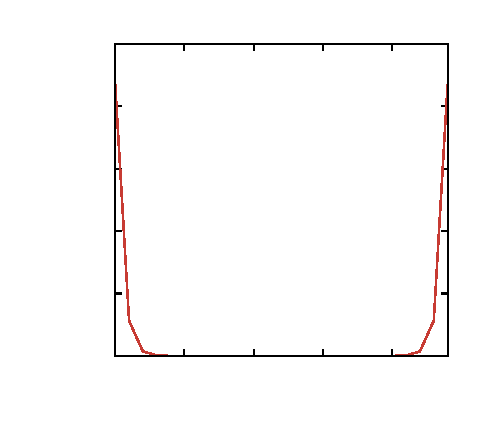
\includegraphics{assets/plots/kitaev_wave/wave36}}%
    \gplfronttext
  \end{picture}%
\endgroup
}
                \caption{$\mu/t = 0$}
                \label{fig:wave_1}
        \end{subfigure}%
        \hspace{\fill}
        \begin{subfigure}[b]{0.4\textwidth}
                    \fontsize{8}{10}\selectfont % zmniejszam czcionke
			    \resizebox{1.0\textwidth}{!}{% GNUPLOT: LaTeX picture with Postscript
\begingroup
  \makeatletter
  \providecommand\color[2][]{%
    \GenericError{(gnuplot) \space\space\space\@spaces}{%
      Package color not loaded in conjunction with
      terminal option `colourtext'%
    }{See the gnuplot documentation for explanation.%
    }{Either use 'blacktext' in gnuplot or load the package
      color.sty in LaTeX.}%
    \renewcommand\color[2][]{}%
  }%
  \providecommand\includegraphics[2][]{%
    \GenericError{(gnuplot) \space\space\space\@spaces}{%
      Package graphicx or graphics not loaded%
    }{See the gnuplot documentation for explanation.%
    }{The gnuplot epslatex terminal needs graphicx.sty or graphics.sty.}%
    \renewcommand\includegraphics[2][]{}%
  }%
  \providecommand\rotatebox[2]{#2}%
  \@ifundefined{ifGPcolor}{%
    \newif\ifGPcolor
    \GPcolortrue
  }{}%
  \@ifundefined{ifGPblacktext}{%
    \newif\ifGPblacktext
    \GPblacktextfalse
  }{}%
  % define a \g@addto@macro without @ in the name:
  \let\gplgaddtomacro\g@addto@macro
  % define empty templates for all commands taking text:
  \gdef\gplbacktext{}%
  \gdef\gplfronttext{}%
  \makeatother
  \ifGPblacktext
    % no textcolor at all
    \def\colorrgb#1{}%
    \def\colorgray#1{}%
  \else
    % gray or color?
    \ifGPcolor
      \def\colorrgb#1{\color[rgb]{#1}}%
      \def\colorgray#1{\color[gray]{#1}}%
      \expandafter\def\csname LTw\endcsname{\color{white}}%
      \expandafter\def\csname LTb\endcsname{\color{black}}%
      \expandafter\def\csname LTa\endcsname{\color{black}}%
      \expandafter\def\csname LT0\endcsname{\color[rgb]{1,0,0}}%
      \expandafter\def\csname LT1\endcsname{\color[rgb]{0,1,0}}%
      \expandafter\def\csname LT2\endcsname{\color[rgb]{0,0,1}}%
      \expandafter\def\csname LT3\endcsname{\color[rgb]{1,0,1}}%
      \expandafter\def\csname LT4\endcsname{\color[rgb]{0,1,1}}%
      \expandafter\def\csname LT5\endcsname{\color[rgb]{1,1,0}}%
      \expandafter\def\csname LT6\endcsname{\color[rgb]{0,0,0}}%
      \expandafter\def\csname LT7\endcsname{\color[rgb]{1,0.3,0}}%
      \expandafter\def\csname LT8\endcsname{\color[rgb]{0.5,0.5,0.5}}%
    \else
      % gray
      \def\colorrgb#1{\color{black}}%
      \def\colorgray#1{\color[gray]{#1}}%
      \expandafter\def\csname LTw\endcsname{\color{white}}%
      \expandafter\def\csname LTb\endcsname{\color{black}}%
      \expandafter\def\csname LTa\endcsname{\color{black}}%
      \expandafter\def\csname LT0\endcsname{\color{black}}%
      \expandafter\def\csname LT1\endcsname{\color{black}}%
      \expandafter\def\csname LT2\endcsname{\color{black}}%
      \expandafter\def\csname LT3\endcsname{\color{black}}%
      \expandafter\def\csname LT4\endcsname{\color{black}}%
      \expandafter\def\csname LT5\endcsname{\color{black}}%
      \expandafter\def\csname LT6\endcsname{\color{black}}%
      \expandafter\def\csname LT7\endcsname{\color{black}}%
      \expandafter\def\csname LT8\endcsname{\color{black}}%
    \fi
  \fi
    \setlength{\unitlength}{0.0500bp}%
    \ifx\gptboxheight\undefined%
      \newlength{\gptboxheight}%
      \newlength{\gptboxwidth}%
      \newsavebox{\gptboxtext}%
    \fi%
    \setlength{\fboxrule}{0.5pt}%
    \setlength{\fboxsep}{1pt}%
\begin{picture}(4534.00,3968.00)%
    \gplgaddtomacro\gplbacktext{%
      \csname LTb\endcsname%
      \put(814,704){\makebox(0,0)[r]{\strut{}$0$}}%
      \put(814,1304){\makebox(0,0)[r]{\strut{}$0.1$}}%
      \put(814,1904){\makebox(0,0)[r]{\strut{}$0.2$}}%
      \put(814,2503){\makebox(0,0)[r]{\strut{}$0.3$}}%
      \put(814,3103){\makebox(0,0)[r]{\strut{}$0.4$}}%
      \put(814,3703){\makebox(0,0)[r]{\strut{}$0.5$}}%
      \put(946,484){\makebox(0,0){\strut{}$0$}}%
      \put(1611,484){\makebox(0,0){\strut{}$5$}}%
      \put(2276,484){\makebox(0,0){\strut{}$10$}}%
      \put(2940,484){\makebox(0,0){\strut{}$15$}}%
      \put(3605,484){\makebox(0,0){\strut{}$20$}}%
    }%
    \gplgaddtomacro\gplfronttext{%
      \csname LTb\endcsname%
      \put(176,2203){\rotatebox{-270}{\makebox(0,0){\strut{}$|u|^2 + |v|^2$}}}%
      \put(2541,154){\makebox(0,0){\strut{}$n$}}%
    }%
    \gplbacktext
    \put(0,0){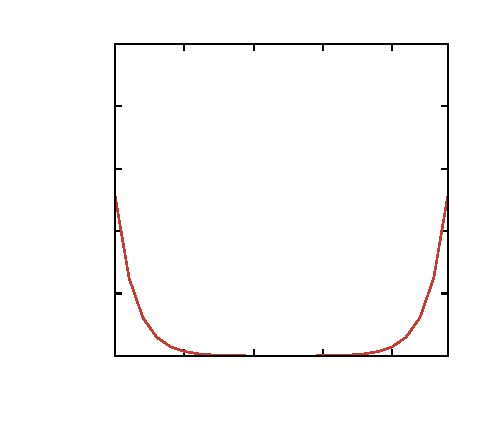
\includegraphics{assets/plots/kitaev_wave/wave70}}%
    \gplfronttext
  \end{picture}%
\endgroup
}
                \caption{$\mu/t = 1,4$}
                \label{fig:wave_2}
        \end{subfigure}%
        \hspace{\fill}
        \begin{subfigure}[b]{0.4\textwidth}
                    \fontsize{8}{10}\selectfont % zmniejszam czcionke
			    \resizebox{1.0\textwidth}{!}{% GNUPLOT: LaTeX picture with Postscript
\begingroup
  \makeatletter
  \providecommand\color[2][]{%
    \GenericError{(gnuplot) \space\space\space\@spaces}{%
      Package color not loaded in conjunction with
      terminal option `colourtext'%
    }{See the gnuplot documentation for explanation.%
    }{Either use 'blacktext' in gnuplot or load the package
      color.sty in LaTeX.}%
    \renewcommand\color[2][]{}%
  }%
  \providecommand\includegraphics[2][]{%
    \GenericError{(gnuplot) \space\space\space\@spaces}{%
      Package graphicx or graphics not loaded%
    }{See the gnuplot documentation for explanation.%
    }{The gnuplot epslatex terminal needs graphicx.sty or graphics.sty.}%
    \renewcommand\includegraphics[2][]{}%
  }%
  \providecommand\rotatebox[2]{#2}%
  \@ifundefined{ifGPcolor}{%
    \newif\ifGPcolor
    \GPcolortrue
  }{}%
  \@ifundefined{ifGPblacktext}{%
    \newif\ifGPblacktext
    \GPblacktextfalse
  }{}%
  % define a \g@addto@macro without @ in the name:
  \let\gplgaddtomacro\g@addto@macro
  % define empty templates for all commands taking text:
  \gdef\gplbacktext{}%
  \gdef\gplfronttext{}%
  \makeatother
  \ifGPblacktext
    % no textcolor at all
    \def\colorrgb#1{}%
    \def\colorgray#1{}%
  \else
    % gray or color?
    \ifGPcolor
      \def\colorrgb#1{\color[rgb]{#1}}%
      \def\colorgray#1{\color[gray]{#1}}%
      \expandafter\def\csname LTw\endcsname{\color{white}}%
      \expandafter\def\csname LTb\endcsname{\color{black}}%
      \expandafter\def\csname LTa\endcsname{\color{black}}%
      \expandafter\def\csname LT0\endcsname{\color[rgb]{1,0,0}}%
      \expandafter\def\csname LT1\endcsname{\color[rgb]{0,1,0}}%
      \expandafter\def\csname LT2\endcsname{\color[rgb]{0,0,1}}%
      \expandafter\def\csname LT3\endcsname{\color[rgb]{1,0,1}}%
      \expandafter\def\csname LT4\endcsname{\color[rgb]{0,1,1}}%
      \expandafter\def\csname LT5\endcsname{\color[rgb]{1,1,0}}%
      \expandafter\def\csname LT6\endcsname{\color[rgb]{0,0,0}}%
      \expandafter\def\csname LT7\endcsname{\color[rgb]{1,0.3,0}}%
      \expandafter\def\csname LT8\endcsname{\color[rgb]{0.5,0.5,0.5}}%
    \else
      % gray
      \def\colorrgb#1{\color{black}}%
      \def\colorgray#1{\color[gray]{#1}}%
      \expandafter\def\csname LTw\endcsname{\color{white}}%
      \expandafter\def\csname LTb\endcsname{\color{black}}%
      \expandafter\def\csname LTa\endcsname{\color{black}}%
      \expandafter\def\csname LT0\endcsname{\color{black}}%
      \expandafter\def\csname LT1\endcsname{\color{black}}%
      \expandafter\def\csname LT2\endcsname{\color{black}}%
      \expandafter\def\csname LT3\endcsname{\color{black}}%
      \expandafter\def\csname LT4\endcsname{\color{black}}%
      \expandafter\def\csname LT5\endcsname{\color{black}}%
      \expandafter\def\csname LT6\endcsname{\color{black}}%
      \expandafter\def\csname LT7\endcsname{\color{black}}%
      \expandafter\def\csname LT8\endcsname{\color{black}}%
    \fi
  \fi
    \setlength{\unitlength}{0.0500bp}%
    \ifx\gptboxheight\undefined%
      \newlength{\gptboxheight}%
      \newlength{\gptboxwidth}%
      \newsavebox{\gptboxtext}%
    \fi%
    \setlength{\fboxrule}{0.5pt}%
    \setlength{\fboxsep}{1pt}%
\begin{picture}(4534.00,3968.00)%
    \gplgaddtomacro\gplbacktext{%
      \csname LTb\endcsname%
      \put(814,704){\makebox(0,0)[r]{\strut{}$0$}}%
      \put(814,1304){\makebox(0,0)[r]{\strut{}$0.1$}}%
      \put(814,1904){\makebox(0,0)[r]{\strut{}$0.2$}}%
      \put(814,2503){\makebox(0,0)[r]{\strut{}$0.3$}}%
      \put(814,3103){\makebox(0,0)[r]{\strut{}$0.4$}}%
      \put(814,3703){\makebox(0,0)[r]{\strut{}$0.5$}}%
      \put(946,484){\makebox(0,0){\strut{}$0$}}%
      \put(1611,484){\makebox(0,0){\strut{}$5$}}%
      \put(2276,484){\makebox(0,0){\strut{}$10$}}%
      \put(2940,484){\makebox(0,0){\strut{}$15$}}%
      \put(3605,484){\makebox(0,0){\strut{}$20$}}%
    }%
    \gplgaddtomacro\gplfronttext{%
      \csname LTb\endcsname%
      \put(176,2203){\rotatebox{-270}{\makebox(0,0){\strut{}$|u|^2 + |v|^2$}}}%
      \put(2541,154){\makebox(0,0){\strut{}$n$}}%
    }%
    \gplbacktext
    \put(0,0){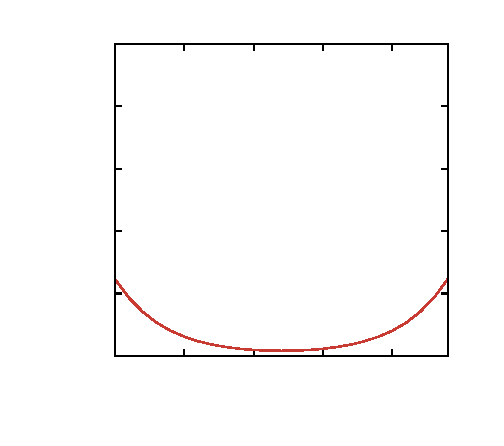
\includegraphics{assets/plots/kitaev_wave/wave87}}%
    \gplfronttext
  \end{picture}%
\endgroup
}
                \caption{$\mu/t = 1,75$}
                \label{fig:wave_3}
        \end{subfigure}%
        \hspace{\fill}
        \begin{subfigure}[b]{0.4\textwidth}
                    \fontsize{8}{10}\selectfont % zmniejszam czcionke
			    \resizebox{1.0\textwidth}{!}{% GNUPLOT: LaTeX picture with Postscript
\begingroup
  \makeatletter
  \providecommand\color[2][]{%
    \GenericError{(gnuplot) \space\space\space\@spaces}{%
      Package color not loaded in conjunction with
      terminal option `colourtext'%
    }{See the gnuplot documentation for explanation.%
    }{Either use 'blacktext' in gnuplot or load the package
      color.sty in LaTeX.}%
    \renewcommand\color[2][]{}%
  }%
  \providecommand\includegraphics[2][]{%
    \GenericError{(gnuplot) \space\space\space\@spaces}{%
      Package graphicx or graphics not loaded%
    }{See the gnuplot documentation for explanation.%
    }{The gnuplot epslatex terminal needs graphicx.sty or graphics.sty.}%
    \renewcommand\includegraphics[2][]{}%
  }%
  \providecommand\rotatebox[2]{#2}%
  \@ifundefined{ifGPcolor}{%
    \newif\ifGPcolor
    \GPcolortrue
  }{}%
  \@ifundefined{ifGPblacktext}{%
    \newif\ifGPblacktext
    \GPblacktextfalse
  }{}%
  % define a \g@addto@macro without @ in the name:
  \let\gplgaddtomacro\g@addto@macro
  % define empty templates for all commands taking text:
  \gdef\gplbacktext{}%
  \gdef\gplfronttext{}%
  \makeatother
  \ifGPblacktext
    % no textcolor at all
    \def\colorrgb#1{}%
    \def\colorgray#1{}%
  \else
    % gray or color?
    \ifGPcolor
      \def\colorrgb#1{\color[rgb]{#1}}%
      \def\colorgray#1{\color[gray]{#1}}%
      \expandafter\def\csname LTw\endcsname{\color{white}}%
      \expandafter\def\csname LTb\endcsname{\color{black}}%
      \expandafter\def\csname LTa\endcsname{\color{black}}%
      \expandafter\def\csname LT0\endcsname{\color[rgb]{1,0,0}}%
      \expandafter\def\csname LT1\endcsname{\color[rgb]{0,1,0}}%
      \expandafter\def\csname LT2\endcsname{\color[rgb]{0,0,1}}%
      \expandafter\def\csname LT3\endcsname{\color[rgb]{1,0,1}}%
      \expandafter\def\csname LT4\endcsname{\color[rgb]{0,1,1}}%
      \expandafter\def\csname LT5\endcsname{\color[rgb]{1,1,0}}%
      \expandafter\def\csname LT6\endcsname{\color[rgb]{0,0,0}}%
      \expandafter\def\csname LT7\endcsname{\color[rgb]{1,0.3,0}}%
      \expandafter\def\csname LT8\endcsname{\color[rgb]{0.5,0.5,0.5}}%
    \else
      % gray
      \def\colorrgb#1{\color{black}}%
      \def\colorgray#1{\color[gray]{#1}}%
      \expandafter\def\csname LTw\endcsname{\color{white}}%
      \expandafter\def\csname LTb\endcsname{\color{black}}%
      \expandafter\def\csname LTa\endcsname{\color{black}}%
      \expandafter\def\csname LT0\endcsname{\color{black}}%
      \expandafter\def\csname LT1\endcsname{\color{black}}%
      \expandafter\def\csname LT2\endcsname{\color{black}}%
      \expandafter\def\csname LT3\endcsname{\color{black}}%
      \expandafter\def\csname LT4\endcsname{\color{black}}%
      \expandafter\def\csname LT5\endcsname{\color{black}}%
      \expandafter\def\csname LT6\endcsname{\color{black}}%
      \expandafter\def\csname LT7\endcsname{\color{black}}%
      \expandafter\def\csname LT8\endcsname{\color{black}}%
    \fi
  \fi
    \setlength{\unitlength}{0.0500bp}%
    \ifx\gptboxheight\undefined%
      \newlength{\gptboxheight}%
      \newlength{\gptboxwidth}%
      \newsavebox{\gptboxtext}%
    \fi%
    \setlength{\fboxrule}{0.5pt}%
    \setlength{\fboxsep}{1pt}%
\begin{picture}(4534.00,3968.00)%
    \gplgaddtomacro\gplbacktext{%
      \csname LTb\endcsname%
      \put(814,704){\makebox(0,0)[r]{\strut{}$0$}}%
      \put(814,1304){\makebox(0,0)[r]{\strut{}$0.1$}}%
      \put(814,1904){\makebox(0,0)[r]{\strut{}$0.2$}}%
      \put(814,2503){\makebox(0,0)[r]{\strut{}$0.3$}}%
      \put(814,3103){\makebox(0,0)[r]{\strut{}$0.4$}}%
      \put(814,3703){\makebox(0,0)[r]{\strut{}$0.5$}}%
      \put(946,484){\makebox(0,0){\strut{}$0$}}%
      \put(1611,484){\makebox(0,0){\strut{}$5$}}%
      \put(2276,484){\makebox(0,0){\strut{}$10$}}%
      \put(2940,484){\makebox(0,0){\strut{}$15$}}%
      \put(3605,484){\makebox(0,0){\strut{}$20$}}%
    }%
    \gplgaddtomacro\gplfronttext{%
      \csname LTb\endcsname%
      \put(176,2203){\rotatebox{-270}{\makebox(0,0){\strut{}$|u|^2 + |v|^2$}}}%
      \put(2541,154){\makebox(0,0){\strut{}$n$}}%
    }%
    \gplbacktext
    \put(0,0){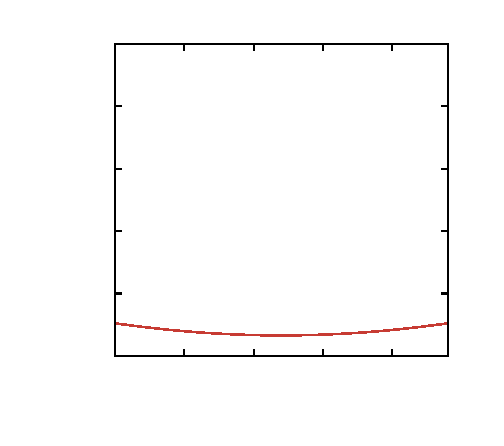
\includegraphics{assets/plots/kitaev_wave/wave97}}%
    \gplfronttext
  \end{picture}%
\endgroup
}
                \caption{$\mu/t = 1,95$}
                \label{fig:wave_4}
        \end{subfigure}
		\hspace{\fill}
        \begin{subfigure}[b]{0.4\textwidth}
	            \fontsize{8}{10}\selectfont % zmniejszam czcionke
			    \resizebox{1.0\textwidth}{!}{% GNUPLOT: LaTeX picture with Postscript
\begingroup
  \makeatletter
  \providecommand\color[2][]{%
    \GenericError{(gnuplot) \space\space\space\@spaces}{%
      Package color not loaded in conjunction with
      terminal option `colourtext'%
    }{See the gnuplot documentation for explanation.%
    }{Either use 'blacktext' in gnuplot or load the package
      color.sty in LaTeX.}%
    \renewcommand\color[2][]{}%
  }%
  \providecommand\includegraphics[2][]{%
    \GenericError{(gnuplot) \space\space\space\@spaces}{%
      Package graphicx or graphics not loaded%
    }{See the gnuplot documentation for explanation.%
    }{The gnuplot epslatex terminal needs graphicx.sty or graphics.sty.}%
    \renewcommand\includegraphics[2][]{}%
  }%
  \providecommand\rotatebox[2]{#2}%
  \@ifundefined{ifGPcolor}{%
    \newif\ifGPcolor
    \GPcolortrue
  }{}%
  \@ifundefined{ifGPblacktext}{%
    \newif\ifGPblacktext
    \GPblacktextfalse
  }{}%
  % define a \g@addto@macro without @ in the name:
  \let\gplgaddtomacro\g@addto@macro
  % define empty templates for all commands taking text:
  \gdef\gplbacktext{}%
  \gdef\gplfronttext{}%
  \makeatother
  \ifGPblacktext
    % no textcolor at all
    \def\colorrgb#1{}%
    \def\colorgray#1{}%
  \else
    % gray or color?
    \ifGPcolor
      \def\colorrgb#1{\color[rgb]{#1}}%
      \def\colorgray#1{\color[gray]{#1}}%
      \expandafter\def\csname LTw\endcsname{\color{white}}%
      \expandafter\def\csname LTb\endcsname{\color{black}}%
      \expandafter\def\csname LTa\endcsname{\color{black}}%
      \expandafter\def\csname LT0\endcsname{\color[rgb]{1,0,0}}%
      \expandafter\def\csname LT1\endcsname{\color[rgb]{0,1,0}}%
      \expandafter\def\csname LT2\endcsname{\color[rgb]{0,0,1}}%
      \expandafter\def\csname LT3\endcsname{\color[rgb]{1,0,1}}%
      \expandafter\def\csname LT4\endcsname{\color[rgb]{0,1,1}}%
      \expandafter\def\csname LT5\endcsname{\color[rgb]{1,1,0}}%
      \expandafter\def\csname LT6\endcsname{\color[rgb]{0,0,0}}%
      \expandafter\def\csname LT7\endcsname{\color[rgb]{1,0.3,0}}%
      \expandafter\def\csname LT8\endcsname{\color[rgb]{0.5,0.5,0.5}}%
    \else
      % gray
      \def\colorrgb#1{\color{black}}%
      \def\colorgray#1{\color[gray]{#1}}%
      \expandafter\def\csname LTw\endcsname{\color{white}}%
      \expandafter\def\csname LTb\endcsname{\color{black}}%
      \expandafter\def\csname LTa\endcsname{\color{black}}%
      \expandafter\def\csname LT0\endcsname{\color{black}}%
      \expandafter\def\csname LT1\endcsname{\color{black}}%
      \expandafter\def\csname LT2\endcsname{\color{black}}%
      \expandafter\def\csname LT3\endcsname{\color{black}}%
      \expandafter\def\csname LT4\endcsname{\color{black}}%
      \expandafter\def\csname LT5\endcsname{\color{black}}%
      \expandafter\def\csname LT6\endcsname{\color{black}}%
      \expandafter\def\csname LT7\endcsname{\color{black}}%
      \expandafter\def\csname LT8\endcsname{\color{black}}%
    \fi
  \fi
    \setlength{\unitlength}{0.0500bp}%
    \ifx\gptboxheight\undefined%
      \newlength{\gptboxheight}%
      \newlength{\gptboxwidth}%
      \newsavebox{\gptboxtext}%
    \fi%
    \setlength{\fboxrule}{0.5pt}%
    \setlength{\fboxsep}{1pt}%
\begin{picture}(4534.00,3968.00)%
    \gplgaddtomacro\gplbacktext{%
      \csname LTb\endcsname%
      \put(814,704){\makebox(0,0)[r]{\strut{}$0$}}%
      \put(814,1304){\makebox(0,0)[r]{\strut{}$0.1$}}%
      \put(814,1904){\makebox(0,0)[r]{\strut{}$0.2$}}%
      \put(814,2503){\makebox(0,0)[r]{\strut{}$0.3$}}%
      \put(814,3103){\makebox(0,0)[r]{\strut{}$0.4$}}%
      \put(814,3703){\makebox(0,0)[r]{\strut{}$0.5$}}%
      \put(946,484){\makebox(0,0){\strut{}$0$}}%
      \put(1611,484){\makebox(0,0){\strut{}$5$}}%
      \put(2276,484){\makebox(0,0){\strut{}$10$}}%
      \put(2940,484){\makebox(0,0){\strut{}$15$}}%
      \put(3605,484){\makebox(0,0){\strut{}$20$}}%
    }%
    \gplgaddtomacro\gplfronttext{%
      \csname LTb\endcsname%
      \put(176,2203){\rotatebox{-270}{\makebox(0,0){\strut{}$|u|^2 + |v|^2$}}}%
      \put(2541,154){\makebox(0,0){\strut{}$n$}}%
    }%
    \gplbacktext
    \put(0,0){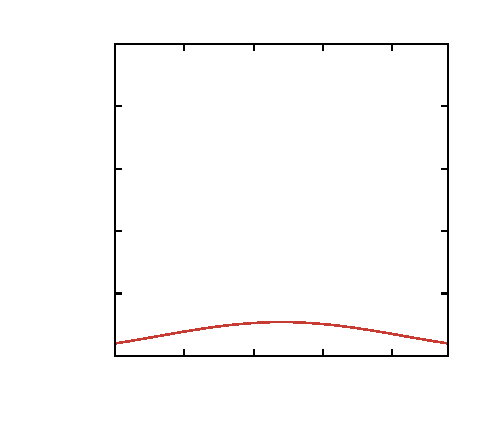
\includegraphics{assets/plots/kitaev_wave/wave108}}%
    \gplfronttext
  \end{picture}%
\endgroup
}
                \caption{$\mu/t = 2,20$}
                \label{fig:wave_5}
        \end{subfigure}
		\hspace{\fill}
        \begin{subfigure}[b]{0.4\textwidth}
	            \fontsize{8}{10}\selectfont % zmniejszam czcionke
			    \resizebox{1.0\textwidth}{!}{% GNUPLOT: LaTeX picture with Postscript
\begingroup
  \makeatletter
  \providecommand\color[2][]{%
    \GenericError{(gnuplot) \space\space\space\@spaces}{%
      Package color not loaded in conjunction with
      terminal option `colourtext'%
    }{See the gnuplot documentation for explanation.%
    }{Either use 'blacktext' in gnuplot or load the package
      color.sty in LaTeX.}%
    \renewcommand\color[2][]{}%
  }%
  \providecommand\includegraphics[2][]{%
    \GenericError{(gnuplot) \space\space\space\@spaces}{%
      Package graphicx or graphics not loaded%
    }{See the gnuplot documentation for explanation.%
    }{The gnuplot epslatex terminal needs graphicx.sty or graphics.sty.}%
    \renewcommand\includegraphics[2][]{}%
  }%
  \providecommand\rotatebox[2]{#2}%
  \@ifundefined{ifGPcolor}{%
    \newif\ifGPcolor
    \GPcolortrue
  }{}%
  \@ifundefined{ifGPblacktext}{%
    \newif\ifGPblacktext
    \GPblacktextfalse
  }{}%
  % define a \g@addto@macro without @ in the name:
  \let\gplgaddtomacro\g@addto@macro
  % define empty templates for all commands taking text:
  \gdef\gplbacktext{}%
  \gdef\gplfronttext{}%
  \makeatother
  \ifGPblacktext
    % no textcolor at all
    \def\colorrgb#1{}%
    \def\colorgray#1{}%
  \else
    % gray or color?
    \ifGPcolor
      \def\colorrgb#1{\color[rgb]{#1}}%
      \def\colorgray#1{\color[gray]{#1}}%
      \expandafter\def\csname LTw\endcsname{\color{white}}%
      \expandafter\def\csname LTb\endcsname{\color{black}}%
      \expandafter\def\csname LTa\endcsname{\color{black}}%
      \expandafter\def\csname LT0\endcsname{\color[rgb]{1,0,0}}%
      \expandafter\def\csname LT1\endcsname{\color[rgb]{0,1,0}}%
      \expandafter\def\csname LT2\endcsname{\color[rgb]{0,0,1}}%
      \expandafter\def\csname LT3\endcsname{\color[rgb]{1,0,1}}%
      \expandafter\def\csname LT4\endcsname{\color[rgb]{0,1,1}}%
      \expandafter\def\csname LT5\endcsname{\color[rgb]{1,1,0}}%
      \expandafter\def\csname LT6\endcsname{\color[rgb]{0,0,0}}%
      \expandafter\def\csname LT7\endcsname{\color[rgb]{1,0.3,0}}%
      \expandafter\def\csname LT8\endcsname{\color[rgb]{0.5,0.5,0.5}}%
    \else
      % gray
      \def\colorrgb#1{\color{black}}%
      \def\colorgray#1{\color[gray]{#1}}%
      \expandafter\def\csname LTw\endcsname{\color{white}}%
      \expandafter\def\csname LTb\endcsname{\color{black}}%
      \expandafter\def\csname LTa\endcsname{\color{black}}%
      \expandafter\def\csname LT0\endcsname{\color{black}}%
      \expandafter\def\csname LT1\endcsname{\color{black}}%
      \expandafter\def\csname LT2\endcsname{\color{black}}%
      \expandafter\def\csname LT3\endcsname{\color{black}}%
      \expandafter\def\csname LT4\endcsname{\color{black}}%
      \expandafter\def\csname LT5\endcsname{\color{black}}%
      \expandafter\def\csname LT6\endcsname{\color{black}}%
      \expandafter\def\csname LT7\endcsname{\color{black}}%
      \expandafter\def\csname LT8\endcsname{\color{black}}%
    \fi
  \fi
    \setlength{\unitlength}{0.0500bp}%
    \ifx\gptboxheight\undefined%
      \newlength{\gptboxheight}%
      \newlength{\gptboxwidth}%
      \newsavebox{\gptboxtext}%
    \fi%
    \setlength{\fboxrule}{0.5pt}%
    \setlength{\fboxsep}{1pt}%
\begin{picture}(4534.00,3968.00)%
    \gplgaddtomacro\gplbacktext{%
      \csname LTb\endcsname%
      \put(814,704){\makebox(0,0)[r]{\strut{}$0$}}%
      \put(814,1304){\makebox(0,0)[r]{\strut{}$0.1$}}%
      \put(814,1904){\makebox(0,0)[r]{\strut{}$0.2$}}%
      \put(814,2503){\makebox(0,0)[r]{\strut{}$0.3$}}%
      \put(814,3103){\makebox(0,0)[r]{\strut{}$0.4$}}%
      \put(814,3703){\makebox(0,0)[r]{\strut{}$0.5$}}%
      \put(946,484){\makebox(0,0){\strut{}$0$}}%
      \put(1611,484){\makebox(0,0){\strut{}$5$}}%
      \put(2276,484){\makebox(0,0){\strut{}$10$}}%
      \put(2940,484){\makebox(0,0){\strut{}$15$}}%
      \put(3605,484){\makebox(0,0){\strut{}$20$}}%
    }%
    \gplgaddtomacro\gplfronttext{%
      \csname LTb\endcsname%
      \put(176,2203){\rotatebox{-270}{\makebox(0,0){\strut{}$|u|^2 + |v|^2$}}}%
      \put(2541,154){\makebox(0,0){\strut{}$n$}}%
    }%
    \gplbacktext
    \put(0,0){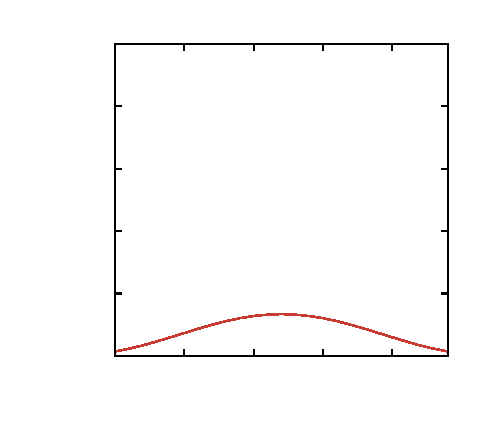
\includegraphics{assets/plots/kitaev_wave/wave128}}%
    \gplfronttext
  \end{picture}%
\endgroup
}
                \caption{$\mu/t = 2,50$}
                \label{fig:wave_6}
        \end{subfigure}

        \caption{Funkcja falowa stanu Majorany w zależności od potencjału chemicznego $\mu$}
\end{figure}


\section{Nanodrut półprzewodnikowy}
\subsection{Założenia}
Model nanodrutu opisany jest Hamiltonianem
\begin{equation}
    H_{\text{wire}} = \left(\frac{\hbar^2 k^2}{2m} + \alpha\sigma_y k - \mu\right)\mathbb{1} \tens \tau_z + B\sigma_z + \Delta\tau_x.
\end{equation}
gdzie: \\ $m$ jest efektywną masą elektronu, \\$B$ - natężeniem polem magnetycznego, \\$\alpha$ parametrem opisującym efekt Rashb'y \\ $\sigma$ - odpowiednią macierzą Pauliego



\subsection{Wyniki pomiarów}
\end{document}














